\documentclass[9pt,twocolumn]{extarticle}

\usepackage[margin=0.45in]{geometry}
\usepackage[T1]{fontenc}
\usepackage[utf8]{inputenc}
\usepackage{lmodern}
\usepackage{microtype}
\usepackage{amsmath}
\usepackage{array}
\usepackage{booktabs}
\usepackage{multirow}
\usepackage{url}
\usepackage{graphicx}
\usepackage{caption}
\usepackage{titlesec}
\usepackage{enumitem}

\linespread{0.9}
\setlength{\parskip}{0.1em}
\setlength{\parindent}{0pt}
\setlength{\columnsep}{0.18in}
\titleformat{\section}{\normalsize\bfseries}{\thesection}{0.5em}{}
\titlespacing*{\section}{0pt}{0.35em}{0.1em}
\setlength{\abovedisplayskip}{3pt}
\setlength{\belowdisplayskip}{3pt}
\setlength{\textfloatsep}{6pt}
\captionsetup{font=footnotesize,labelfont=bf,skip=3pt}
\setlist{nosep,leftmargin=1.2em}
\graphicspath{{figures/}}
\pagestyle{plain}
\raggedbottom
\urlstyle{tt}
\newcommand{\code}[1]{\path{#1}}

\begin{document}

\twocolumn[{\large\bfseries Phase 1: Memory-Aware Agent Edge Serving}\par
\vspace{0.12em}
CSE 291A, Fall 2026, Option 1. November 4, 2026.\par
\vspace{0.18em}
Figures and full tables are in the appendix. The numbers below are means across repeats unless noted otherwise.\par
\vspace{0.5em}]

\section{What we wanted to know}

We wanted to know how a FIFO scheduler performs on one laptop with a fixed KV cache budget, and which problems dominate its performance. Our setup uses a multi-step agent that calls the model, waits on a tool, and then calls the model again with a longer prompt. While the tool is running the model is free, but the KV cache from the previous step still retains useful information, and on a 16 GB laptop that cache is the limited resource. A fixed-concurrency FIFO scheduler can fail here for two main reasons. The first reason is that too few agents are allowed in at once, resulting in idle time. For example, if only one agent is in the system, it finishes a model step and then waits on a tool, and during the wait the model has no other request to run. The model then sits idle when it could be processing other tasks. The second reason is admitting too many agents at once. For example, agent A has already run, so its slot holds the tokens from that call. Agent B then gets the same slot and overwrites them. When A comes back, the new prompt still starts with those same tokens, but the server has to recompute them all over again before it can read the new tool result. We implemented that FIFO in front of one \texttt{llama-server}, on a real agent benchmark and on controlled prompts, to see which of those two effects dominates and what a later policy would have to beat. We do not implement a new policy in this phase.

\section{Implementation}

We ran the experiments on a MacBook Air M4 with 16 GB of unified memory, running macOS 15.3, and the runs were taken on AC power. The model was Qwen3-4B at Q4\_K\_M with thinking disabled, the KV cache had f16 precision, and a token took up roughly 144 KiB. The server was llama.cpp \texttt{llama-server} build 11669. We fixed the build since slot save, restore, and the cache flags can vary across builds. We later repeated the full matrix on an AWS T4 GPU with the same model, build and workloads, and measured run-to-run noise on a second Mac (M5); those numbers are never mixed with the M4 numbers. The server launcher starts a single server process with $P$ slots and a total context budget, typically 24,576 tokens, which is split across the slots. The server allocates the entire KV pool at startup, so its memory usage stays roughly the same when the queue experiences more traffic.

The queue sits in front of that server. It takes steps that are already ready and runs up to $K$ of them in that ready order; it does not keep the order in which the tasks first showed up. A tool wait happens outside the queue, so a task that is blocked on a tool does not hold one of the $K$ permits. An optional cap $J$ restricts how many agent tasks can be in the system at once, and time spent waiting for $J$ counts toward latency. $K$ only limits model calls that are ready to run, while $J$ limits how many whole agents are allowed in.

The live capture is the only place where a real agent runs. We had the agent execute $\tau^{2}$-bench Retail v1.0.1 with the official tools, orchestrator, and environment checker, with local Qwen as the agent and DeepSeek as the user simulator. A small adapter cleans a tool call's JSON: it turns a plain-text tool call into a \texttt{tool\_calls} entry that the Retail benchmark recognizes, but only when the text is a JSON object with a name and an arguments object and the name is an existing Retail tool. Otherwise it leaves the message alone.

\section{Workload}

We sampled 20 eval tasks and 10 dev tasks with seed 291 and kept every task, even the ones that failed. Eval tasks take roughly 2 to 20 model calls, with a median of 11, and the longest prompt in a task is between 5,030 and 9,677 tokens. The environment check passed on only 3 of the 20 eval tasks. The 4B model is weak at this Retail task, but we did not drop these failures. We used the dev tasks only to pick a baseline.

We ran each Retail task once and saved its shape: how many model calls there were, how long each answer was, and how much the prompt grew after each tool result. The 20 eval recordings and the 10 dev recordings are frozen as the workload.

The timed runs did not call DeepSeek and did not run the shop again. Instead, they played the recording back. Suppose a task has already called the model once. The next prompt is that same prompt, plus the tokens the model just wrote in this replay, plus a piece of the saved prompt. We sized that piece in tokens so the prompt grows by the same number of tokens it grew in the live run. The answer length is fixed to the live run too, so one setup cannot look faster by writing a shorter answer. We append the new tokens to the end instead of rewriting the prompt, because the server can reuse the old tokens only if the next request starts with those exact same tokens.

The benchmark runner takes 8 of those saved tasks, which arrive at random times (Poisson, on average about once per minute), and after each model step it simulates a tool with a log-normal delay (median 2 seconds). It then inserts the next step into the FIFO queue. The sweep script restarts the server when the number of slots or the cache flags change, since those are fixed at startup. Repeat 0 is the same 8 tasks, the same arrival times, and the same tool delays for every configuration. Repeat 1 is a different seeded draw of tasks, arrival times, and tool delays. If two configurations differ on repeat 0, that can be attributed to the configuration. If repeat 0 and repeat 1 differ, that can be attributed to a different mix of tasks. Finishing a task means every saved step ran. It does not necessarily mean the customer was actually helped.

We also ran two checks that are not the Retail replay. The micro benchmark used exact lengths: 1K, 4K, and 8K tokens in and 64 or 512 tokens out, with the prompt cache disabled. The cache check measured the continuation after a slot is kept, idle, overwritten, erased, or saved to SSD and restored.

\section{Findings}

\textbf{Rebuilding a long prompt is the slow part.} At $K = 1$, the prefill of 8,192 tokens took 43.6 seconds, about 184 tokens per second. Generating 512 tokens on a 1,024-token prompt took about 23.6 seconds end to end, and only 4.4 seconds of that was prefill. Losing an 8K history therefore costs more than writing the answer: its 43.6 seconds of prefill is as long as generating about 1,160 output tokens (Figure A1).

\textbf{If the slot is still there, that cost almost goes away.} After an 8K prompt, a continuation's prefill took about 0.17 to 0.20 seconds and reused 99.9\% of the input when the slot was retained, idle, or loaded from disk. Overwrite and erase dropped to 0\% reuse and took about 44 seconds. The 8K state took up 1,156 MiB; saving it took only 0.37 seconds and restoring it 0.35 seconds, and these steps combined with prefill took about 0.90 seconds. After save, overwrite, and restore, 64 greedy tokens matched the run that was never interrupted. Saving a slot to disk is cheap on this machine, but recomputing the prefix is not (Table A3).

\textbf{The process does not get bigger when we add load.} llama-server allocates the KV pool up front, so a 24K budget is 3.38 GiB of KV on paper; the process peaks around 3.6 GiB RSS, with about 1.9 GiB still free. Four slots at the same budget use about the same RSS. The memory limit shows up as agents overwriting each other's slots, or as a prompt that does not fit in its slot. It does not show up as RSS climbing with load. With two slots, a returning task finds its whole history 100\% of the time when it is alone, 83\% with two active tasks, 11\% with three, and never with four (Table A4, Figure A3).

\begin{table*}[t]
\centering
\footnotesize
\setlength{\tabcolsep}{5pt}
\caption{M4 retail replays under the default load (24K-token budget, log-normal tool delay with median 2 s, one Poisson arrival per minute). P50 and P95 are averages of the per-run percentiles, and latency only includes tasks that finished. $\pm$ is the standard deviation across repeats, which mostly reflects which tasks each repeat drew. The full table is Table A1.}
\label{tab:main}
\begin{tabular}{@{}lrrrrrr@{}}
\toprule
Setup & Finished & Tasks/min & P50 & P95 & History prefilled again & Full history hit \\
\midrule
2 slots, $K = 2$, no task cap (FIFO) & 24/24 & $0.59 \pm 0.20$ & 318 s & 479 s & 45\% & 58\% \\
2 slots, $K = 2$, at most 2 tasks ($J = 2$) & 24/24 & $0.74 \pm 0.23$ & 152 s & 256 s & 20\% & 96\% \\
2 slots, $K = 2$, no task cap, plus a 3 GiB host prompt cache & 24/24 & $0.53 \pm 0.11$ & 363 s & 532 s & 64\% & 45\% \\
4 slots, $K = 4$, 6K tokens each & 10/24 & $0.42 \pm 0.21$ & 38 s & 68 s & 16\% & 88\% \\
\bottomrule
\end{tabular}
\end{table*}

\textbf{On the M4 retail replays, capping active tasks is the best simple setup, and it is unfair.} Table~\ref{tab:main} compares the main setups.

\textbf{The 4-slot latencies look short because the long tasks are the ones that die.} They fail with ``context size has been exceeded.'' Increasing the context budget to 36K tokens, about 9K per slot, decreased the failures to 3 out of 16 tasks, and that run still does not beat the 2-slot configuration with our task cap. All 25 failed tasks are such overflows, and they stay in every denominator; no request reached the 600-second deadline.

\textbf{The variation across repeats is mostly which tasks were drawn.} Each repeat is a different draw of 8 tasks, and every configuration sees the same 8. One repeat is a long batch: with no cap, the median task took 747 seconds. Another repeat is a short batch, with a median of 50 seconds. On the three repeats the cap is 1.03 times, 0.97 times, and 1.97 times the uncapped FIFO, so it is a big win on one batch and about a tie on the other two. The big win is the batch where tasks overlap the most, 4.4 tasks active under FIFO against 2.4 and 0.7, not only the batch with longer prompts (Table A6).

\textbf{On the long batch, the cap wins by keeping histories in their slots.} With no cap, a task on that batch waits about 292 seconds in the FIFO line, spends about 255 seconds in the model round trip, and finishes after 580 seconds. Most of that model time recomputes old tokens after another agent took the slot, and because every step is longer, the line behind it grows too. At $K = 2$ the round trip also includes time spent sharing the server. With the cap, the line wait is 0, a task waits about 120 seconds to be let in, the round trip falls to about 91 seconds, and the task finishes after 244 seconds. The tool wait stays about 33 seconds either way. On the M4 dev tasks, the 10 we held out, $P = 2$, $K = 2$, $J = 2$ was the best of the four runs (one run each), about 0.91 tasks per minute, and none of the prefill was old tokens being computed again. Uncapped FIFO on those tasks was about 0.45 tasks per minute, and 77\% of the prefill was old tokens. On the M4, Phase 2 therefore has to beat this setup, not only uncapped FIFO.

\textbf{The same cap does not win on a faster GPU.} We also ran the full matrix on an AWS T4, three trials of every run, with arrivals raised to 3.5 tasks per minute so that tasks overlap about as much as on the M4. Histories are lost the same way: with two slots, a returning task finds its whole history 98\% of the time alone, 37\% with three active tasks, and 15\% with four. But on the T4 an 8K re-prefill takes 5.1 seconds instead of 44, and a model step (1.9 seconds) is shorter than a tool wait (2.9 seconds), so the cap mostly leaves the GPU idle while admitted agents wait on tools. The $J = 2$ cap finishes tasks at 0.91, 1.00, and 0.79 times FIFO on the three repeats, and the best fixed cap on the T4 dev tasks is $J = 4$ (1.04 times FIFO). Whether a cap helps depends on how expensive a lost history is compared with a tool wait (Tables A2 and A6, Figure A4).

\textbf{The cap is also unfair to short tasks.} Slowdown is
\begin{equation}
\mathrm{slowdown} = \frac{T_{\mathrm{completion}}}{T_{K=1,J=1} + T_{\mathrm{tool}}}
\end{equation}
\(T_{\mathrm{completion}}\) is how long the task took in that run, \(T_{K=1,J=1}\) is its model time when it runs alone, and \(T_{\mathrm{tool}}\) is its own tool wait. Under the cap, short tasks, split at the median output length, slow down by 9.5 times and long tasks by 1.6 times, because the short ones are waiting to be admitted. With no cap the slowdowns are closer, about 4.5 times for short tasks and 3.4 times for long tasks, and the whole run is slower. The T4 shows the same pattern: short-task slowdown rises from 1.5 under FIFO to 8.5 under $J = 2$ (Figure A6).

\textbf{llama.cpp does not keep a slot for each agent.} Every Retail task starts with the same 4,891-token system prompt and tool schema. llama.cpp picks the idle slot whose cached prompt shares the longest prefix, and when $K = 1$ every slot is idle, so it keeps choosing the same slot and the second slot stays empty. Two active tasks then overwrite each other in that one slot. When a history is lost, the shared prefix usually survives and only the task-specific tail is recomputed. A slot is therefore not reserved for an agent unless we pass \texttt{id\_slot} ourselves.

\textbf{The host prompt cache did not help.} \texttt{-{}-cache-ram 3072} is the 3 GiB row in Table~\ref{tab:main}. On the same eval mixes it was no better than no cache (0.81, 1.00, and 0.99 times FIFO on the three repeats), and on the T4 it matched FIFO exactly.

\textbf{Tool delay and arrival rate change how often agents overwrite each other's old tokens.} With 2 slots and $K = 2$, we first changed only the wait after each model step: no wait, the usual median 2-second wait, and a fixed 15-second wait. Each repeat is a different draw of 8 tasks, so we compared only the repeats where all three waits ran. No wait and the 2-second wait are close, 0.60 and 0.65 tasks per minute respectively, inside the long-batch versus short-batch gap. The 15-second wait is worse: 66\% of the prefill is old tokens computed again, and finished tasks fall to 0.46 per minute. We then changed only how often a new task shows up. At one task every 2 minutes, a task takes 1.3 times as long as running alone, and 92\% of next steps still have the whole previous prompt. At 2 tasks per minute, finished tasks increase to 0.80 per minute, P95 increases to 416 seconds, and only 55\% of next steps still have the whole previous prompt. The one-per-minute number here is 0.65, not 0.59 as in Table~\ref{tab:main}, because only the repeats that all three rates ran are included (Figure A7).

\section{What we plan for Phase 2}

For Phase 2 we want one policy whose decisions come from costs it measures while running, because the best fixed cap is $J = 2$ on the M4 and $J = 4$ on the T4. It has three parts. First, pin each agent to a slot, so $K = 1$ stops leaving a slot unused. Second, run a ready continuation before a new task, with an aging term so a long task cannot wait forever, and admit a new task when the server would otherwise sit idle and the budget can hold the context growth we have actually seen. This is meant to keep the hit rate of the cap while cutting the wait that short tasks pay. Third, when a tool runs long, choose between keeping the slot, saving it to SSD, and dropping it from the measured costs. On the M4 that save is under a second, and an 8K re-prefill is 44 seconds. On the T4 the same save is 8.95 seconds against a 5.1-second re-prefill, so a save pays only when it is written during a long tool wait. We plan to log the decision time and count it in the latency measurement.

We also plan to keep the comparisons on one model, one precision, and the same output lengths. The baselines are a plain FIFO, the best fixed setup checked on dev for each machine ($J = 2$ on the M4 and $J = 4$ on the T4), and \texttt{-{}-cache-ram} as the simple fixed cache, together with queue only, cache only, and both together. We will also rerun the 0.5 per minute arrival and the zero-delay case, where there is little eviction to remove, so the policy should not help much there. A speedup has to show up as less repeated prefill. Dropping tasks or shortening outputs does not count.

\section{Limits}

Eight tasks and three repeats, or two repeats for the 36K run and for the delay and arrival sweeps, mean that P95 only describes these runs. The M4 runs were done once per repeat. On the M5, three trials of repeat 0 on identical inputs varied by 11\% for uncapped FIFO and 2\% for the $J = 2$ cap, and the cap was ahead in every trial, so M4 differences under about 20\% should be read as ties. On the T4, run-to-run variation was at most 1.3\% (Table A5). All runs start from a warm server with empty slots; loading the model takes 0.66 seconds on the M4 and is excluded. RSS under-counts Metal allocations. One launch was on battery; we moved it out of the results and reran it on AC.

\onecolumn
\appendix
\renewcommand{\thesection}{\Alph{section}}
\renewcommand{\thetable}{A\arabic{table}}
\renewcommand{\thefigure}{A\arabic{figure}}
\setcounter{table}{0}

\section{Artifacts and reproduction}

All code, workloads, raw logs and generated reports are in the project repository.

\begin{center}
\footnotesize
\begin{tabular}{@{}ll@{}}
\toprule
Artifact & Location \\
\midrule
FIFO queue, request logging, append-only replay & \code{phase1/core.py} \\
Server launcher ($P$, budget, unified KV, host cache) & \code{phase1/server.py} \\
Live $\tau^2$-bench capture; tool-call normalization & \code{phase1/capture.py}, \code{phase1/adapters.py} \\
Micro, cache and macro suites; admission cap $J$ & \code{phase1/bench.py} \\
Summaries, noise, figures and generated reports & \code{phase1/summarize.py}, \code{phase1/noise.py}, \code{phase1/final.py} \\
Full pipeline (resumable) & \code{scripts/overnight.sh} \\
Frozen workloads (20 eval, 10 dev) & \code{runs/final/workload_eval.json}, \code{runs/final/workload_dev.json} \\
M4 results, generated report and figures & \code{runs/final/}, \code{runs/final-dev/} \\
T4 results, generated report and figures & \code{runs/aws-gpu/}, \code{runs/aws-gpu-dev/}, \code{REPORT.md} \\
T4 arrival-rate calibration pilot & \code{runs/aws-gpu-pilot/} \\
M5 run-to-run noise trials & \code{runs/m5-noise/} \\
\bottomrule
\end{tabular}
\end{center}

Every number in this report is regenerated from the raw logs, without the model or a GPU, by \texttt{python -m phase1.final --results-dir runs/final --main-arrival poisson:1} (M4) and \texttt{--results-dir runs/aws-gpu --main-arrival scaled:3.5} (T4). Each run records its git commit, server command, power state and (on the T4) GPU identity in \code{raw/runs_meta.jsonl}.

\section{Full tables}

\begin{table}[h]
\centering
\footnotesize
\setlength{\tabcolsep}{4pt}
\caption{M4 baselines under the main condition (24K tokens, log-normal tool delay, 1 task/min). Tasks/min is mean $\pm$ SD across repeats, which mostly reflects the task mix of each repeat; other columns are means of per-run values. Latency covers finished tasks only.}
\begin{tabular}{@{}lrrrrrrrr@{}}
\toprule
Configuration & Repeats & Finished & Tasks/min & P50 (s) & P95 (s) & Re-prefill & Full-history hit & Mean slowdown \\
\midrule
$P=1$, $K=1$ & 3 & 24/24 & $0.483 \pm 0.116$ & 382 & 575 & 78.0\% & 26.4\% & 4.61 \\
$P=2$, $K=1$, $J=1$ & 3 & 24/24 & $0.677 \pm 0.197$ & 174 & 280 & 0.0\% & 100.0\% & 7.49 \\
$P=2$, $K=1$, $J=\infty$ & 3 & 24/24 & $0.450 \pm 0.051$ & 412 & 638 & 78.0\% & 25.1\% & 5.15 \\
$P=2$, $K=2$, $J=2$ & 3 & 24/24 & $0.736 \pm 0.228$ & 152 & 256 & 20.0\% & 95.7\% & 5.53 \\
$P=2$, $K=2$, $J=\infty$ (FIFO) & 3 & 24/24 & $0.587 \pm 0.203$ & 318 & 479 & 45.4\% & 57.8\% & 3.98 \\
FIFO + 3 GiB host cache & 3 & 24/24 & $0.532 \pm 0.113$ & 363 & 532 & 63.6\% & 45.0\% & 4.70 \\
$P=4$, $K=4$, 24K & 3 & 10/24 & $0.424 \pm 0.205$ & 38 & 68 & 15.6\% & 87.5\% & 4.23 \\
$P=4$, $K=4$, 36K & 2 & 13/16 & $0.528 \pm 0.141$ & 50 & 169 & 7.1\% & 97.8\% & 1.52 \\
$P=4$ unified, $K=4$, 24K & 3 & 16/24 & $0.465 \pm 0.052$ & 111 & 203 & 31.5\% & 77.3\% & 4.42 \\
\bottomrule
\end{tabular}
\end{table}

\begin{table}[h]
\centering
\footnotesize
\setlength{\tabcolsep}{4pt}
\caption{T4 baselines under the main condition (24K tokens, log-normal tool delay, 3.5 tasks/min). Each row is 3 repeats $\times$ 3 trials $\times$ 8 tasks; tasks/min is mean $\pm$ SD across repeats of the per-repeat trial means.}
\begin{tabular}{@{}lrrrrrr@{}}
\toprule
Configuration & Finished & Tasks/min & P50 (s) & P95 (s) & Full-history hit & Re-prefill \\
\midrule
$P=2$, $K=2$, $J=\infty$ (FIFO) & 72/72 & $2.133 \pm 0.662$ & 65 & 132 & 57\% & 62\% \\
$P=2$, $K=2$, $J=4$ & 72/72 & $2.086 \pm 0.620$ & 64 & 129 & 62\% & 60\% \\
$P=2$, $K=2$, $J=3$ & 72/72 & $2.096 \pm 0.627$ & 59 & 128 & 69\% & 60\% \\
$P=2$, $K=2$, $J=2$ & 72/72 & $1.875 \pm 0.455$ & 73 & 138 & 91\% & 39\% \\
$P=2$, $K=1$, $J=\infty$ & 72/72 & $1.914 \pm 0.546$ & 85 & 147 & 25\% & 79\% \\
$P=2$, $K=1$, $J=1$ & 72/72 & $1.229 \pm 0.086$ & 155 & 241 & 100\% & 0\% \\
$P=1$, $K=1$ & 72/72 & $1.915 \pm 0.547$ & 84 & 147 & 25\% & 79\% \\
FIFO + 3 GiB host cache & 72/72 & $2.135 \pm 0.663$ & 66 & 132 & 57\% & 64\% \\
$P=4$, $K=4$, 24K & 30/72 & $1.246 \pm 0.459$ & 16 & 19 & 82\% & 36\% \\
$P=4$ unified, $K=4$, 24K & 48/72 & $1.511 \pm 0.430$ & 36 & 92 & 79\% & 43\% \\
$P=4$, $K=4$, 36K (R0--R1) & 39/48 & $1.507 \pm 0.429$ & 29 & 102 & 90\% & 47\% \\
\bottomrule
\end{tabular}
\end{table}

\begin{table}[h]
\centering
\footnotesize
\setlength{\tabcolsep}{5pt}
\begin{minipage}[t]{0.48\textwidth}
\centering
\caption{Platform costs. Micro and cache-probe results at $K=1$.}
\begin{tabular}{@{}lrr@{}}
\toprule
& M4 & T4 \\
\midrule
Prefill rate (tokens/s) & 184 & 1,565 \\
Decode rate (tokens/s) & 27 & 66 \\
Re-prefill of 8K history (s) & 44.1 & 5.1 \\
Continuation with slot kept (s) & 0.20 & 0.03 \\
Save 8K slot state (s) & 0.37 & 8.95 \\
Restore 8K slot state (s) & 0.35 & 0.47 \\
Model step / tool time per step (s) & 9.5 / 2.9 & 1.9 / 2.9 \\
Server busy under FIFO & 71\% & 60\% \\
Model load, median (s) & 0.66 & 1.32 \\
\bottomrule
\end{tabular}
\end{minipage}\hfill
\begin{minipage}[t]{0.48\textwidth}
\centering
\caption{Full-history hit rate by number of active tasks at dispatch, pooled over all runs of each server.}
\begin{tabular}{@{}lrrrrr@{}}
\toprule
Active tasks & 1 & 2 & 3 & 4 & 5 \\
\midrule
M4, $P=2$, 24K & 100\% & 83\% & 11\% & 0\% & 0\% \\
M4, $P=4$, 36K & 100\% & 96\% & 92\% & -- & -- \\
T4, $P=2$, 24K & 98\% & 81\% & 37\% & 15\% & 1\% \\
T4, $P=4$, 24K & 97\% & 81\% & 72\% & 69\% & 40\% \\
T4, $P=4$, 36K & 96\% & 94\% & 81\% & 77\% & -- \\
\bottomrule
\end{tabular}

\vspace{0.8em}
\caption{Run-to-run noise on the M5: R0 replayed three times on identical inputs.}
\begin{tabular}{@{}lrrrr@{}}
\toprule
& Trial 1 & Trial 2 & Trial 3 & CV \\
\midrule
FIFO, tasks/min & 0.662 & 0.567 & 0.542 & 11\% \\
$J=2$, tasks/min & 0.739 & 0.732 & 0.764 & 2\% \\
\bottomrule
\end{tabular}
\end{minipage}
\end{table}


\begin{table}[h]
\centering
\footnotesize
\setlength{\tabcolsep}{5pt}
\caption{Completed tasks per minute relative to FIFO ($P=2$, $K=2$, $J=\infty$) on the same tasks, per repeat. T4 values are means of three trials. Throughput counts finished tasks only, so the 4-slot rows also lose tasks to context overflow.}
\begin{tabular}{@{}lrrrrcrrrr@{}}
\toprule
& \multicolumn{4}{c}{M4, 1 task/min, one run per repeat} & & \multicolumn{4}{c}{T4, 3.5 tasks/min, three trials per repeat} \\
\cmidrule(lr){2-5}\cmidrule(lr){7-10}
Configuration & R0 & R1 & R2 & Finished & & R0 & R1 & R2 & Finished \\
\midrule
FIFO, absolute tasks/min & 0.82 & 0.49 & 0.45 & 24/24 & & 2.47 & 1.37 & 2.56 & 72/72 \\
\midrule
$P=2$, $K=2$, $J=4$ & -- & -- & -- & -- & & 1.00 & 1.00 & 0.94 & 72/72 \\
$P=2$, $K=2$, $J=3$ & -- & -- & -- & -- & & 1.00 & 1.00 & 0.96 & 72/72 \\
$P=2$, $K=2$, $J=2$ & 1.03 & 0.97 & \textbf{1.97} & 24/24 & & 0.91 & 1.00 & \textbf{0.79} & 72/72 \\
$P=2$, $K=1$, $J=1$ & 1.01 & 0.93 & 1.65 & 24/24 & & 0.53 & 0.83 & 0.48 & 72/72 \\
$P=2$, $K=1$, $J=\infty$ & 0.62 & 0.89 & 0.90 & 24/24 & & 0.91 & 0.94 & 0.86 & 72/72 \\
FIFO + 3 GiB host prompt cache & 0.81 & 1.00 & 0.99 & 24/24 & & 1.00 & 1.00 & 1.00 & 72/72 \\
$P=4$, $K=4$, 6K tokens per slot & 0.42 & 0.55 & 1.45 & 10/24 & & 0.44 & 0.64 & 0.69 & 30/72 \\
\bottomrule
\end{tabular}
\end{table}

\clearpage
\section{Figures}

\begin{figure}[h]
\centering
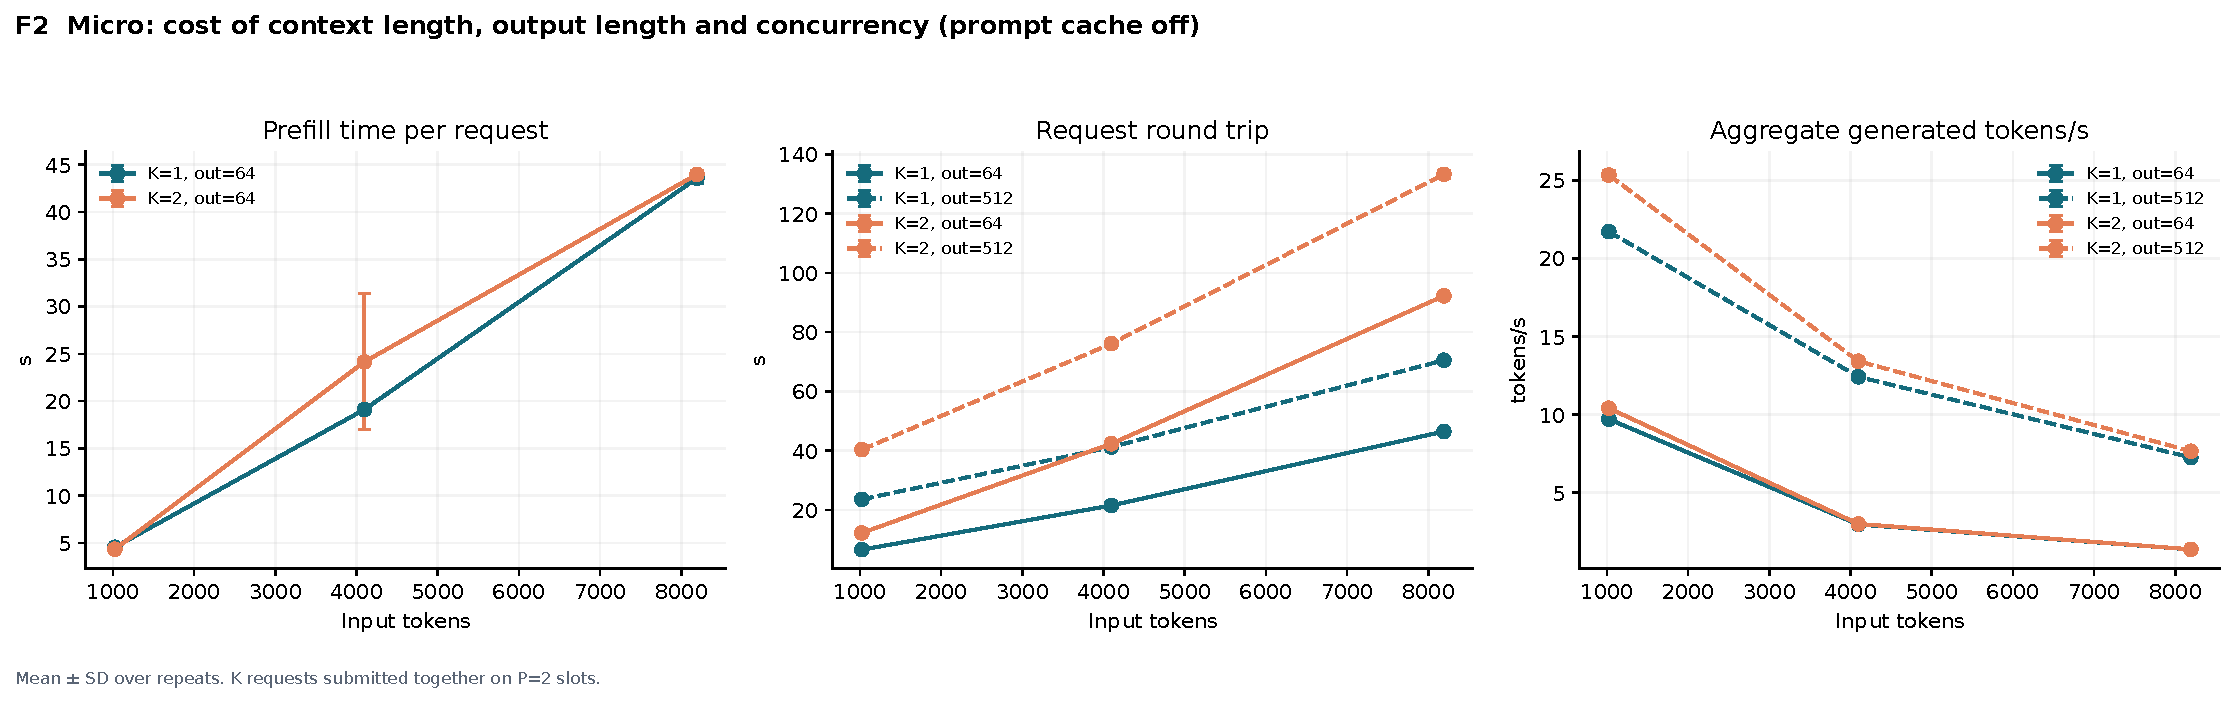
\includegraphics[width=\textwidth]{m4_f02_micro.pdf}
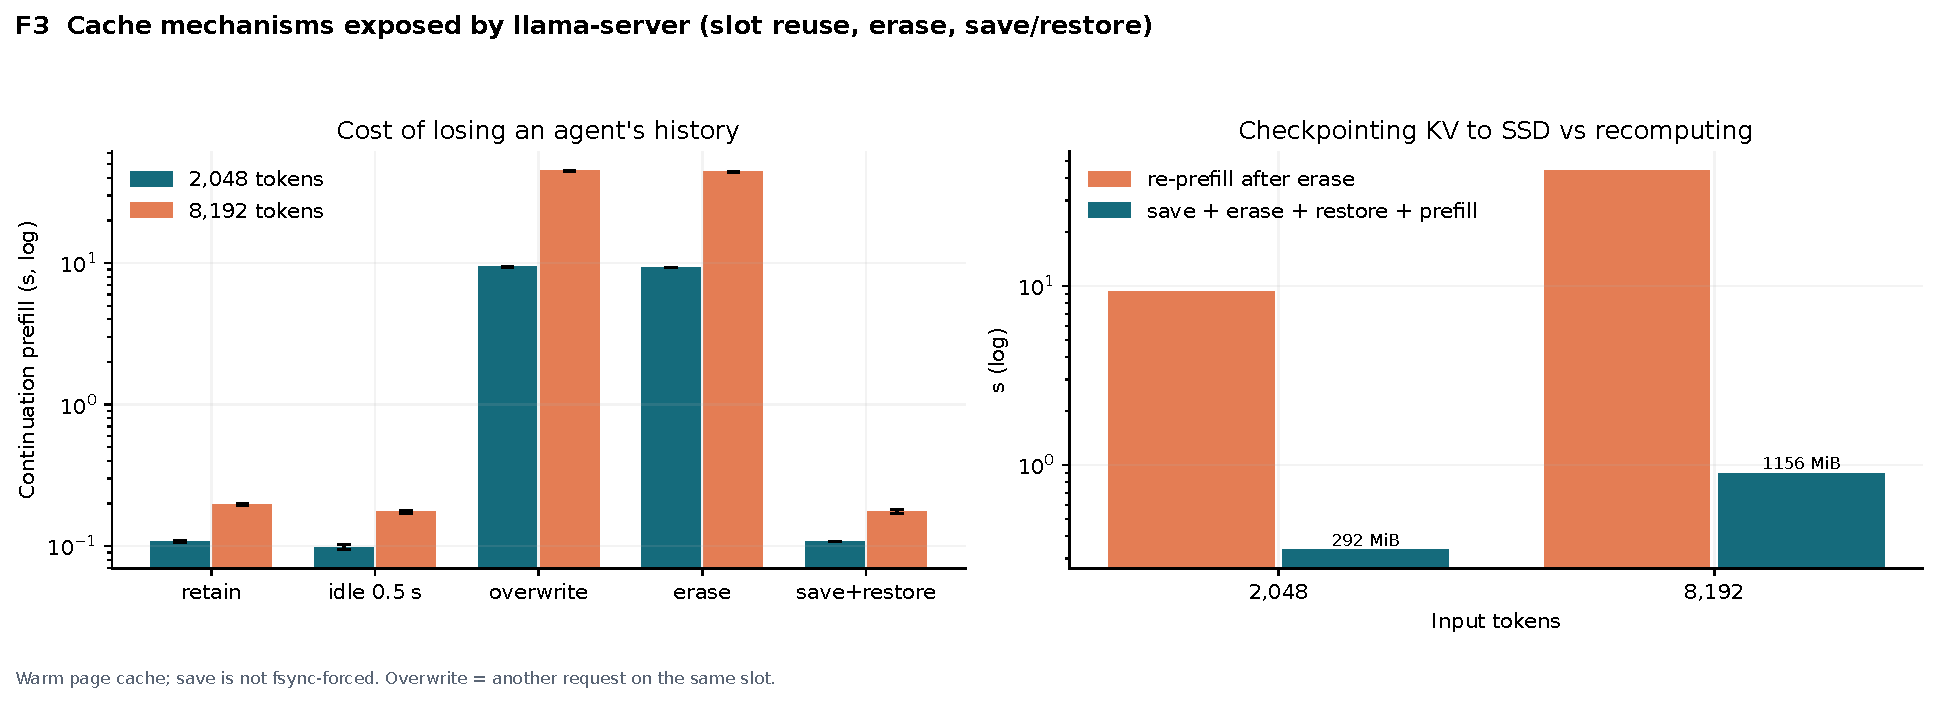
\includegraphics[width=\textwidth]{m4_f03_cache.pdf}
\caption{M4 micro benchmark and cache probe: prefill dominates long contexts, and a kept, idle or restored slot removes it.}
\end{figure}

\begin{figure}[h]
\centering
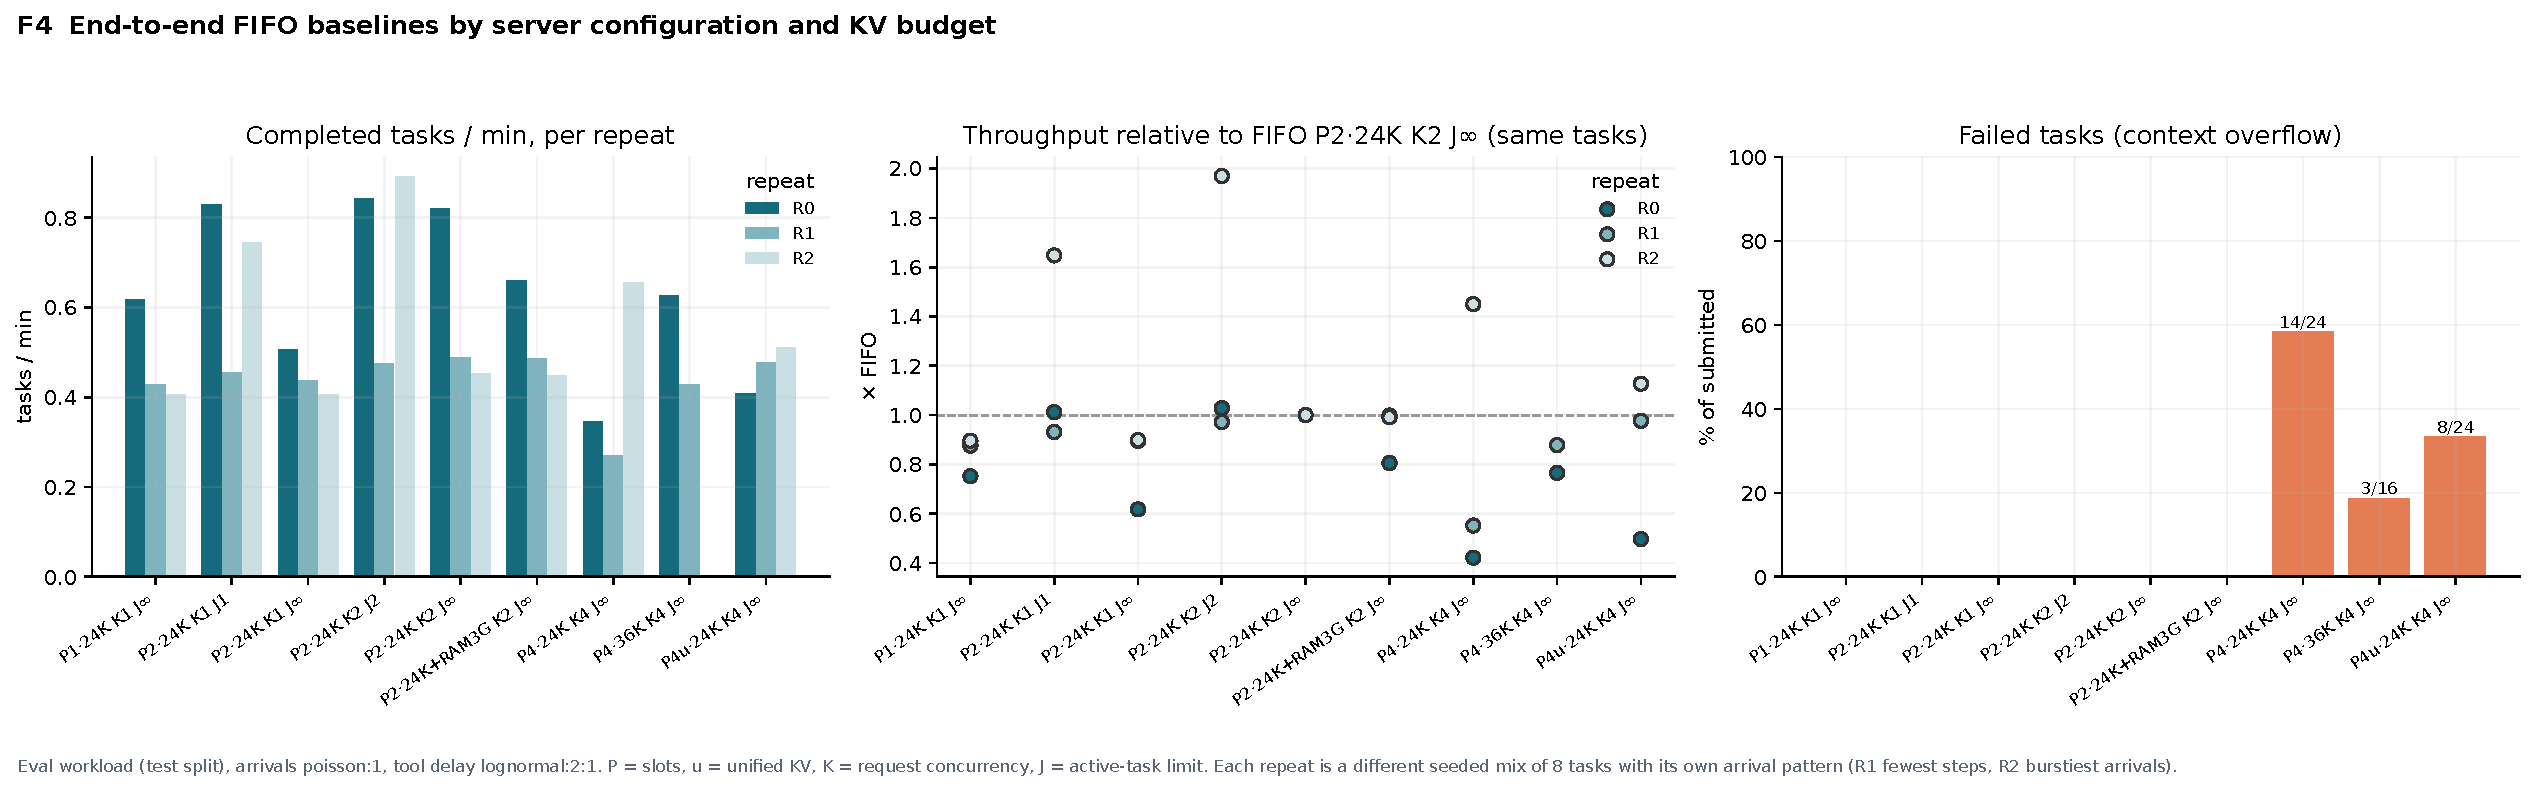
\includegraphics[width=\textwidth]{m4_f04_main.pdf}
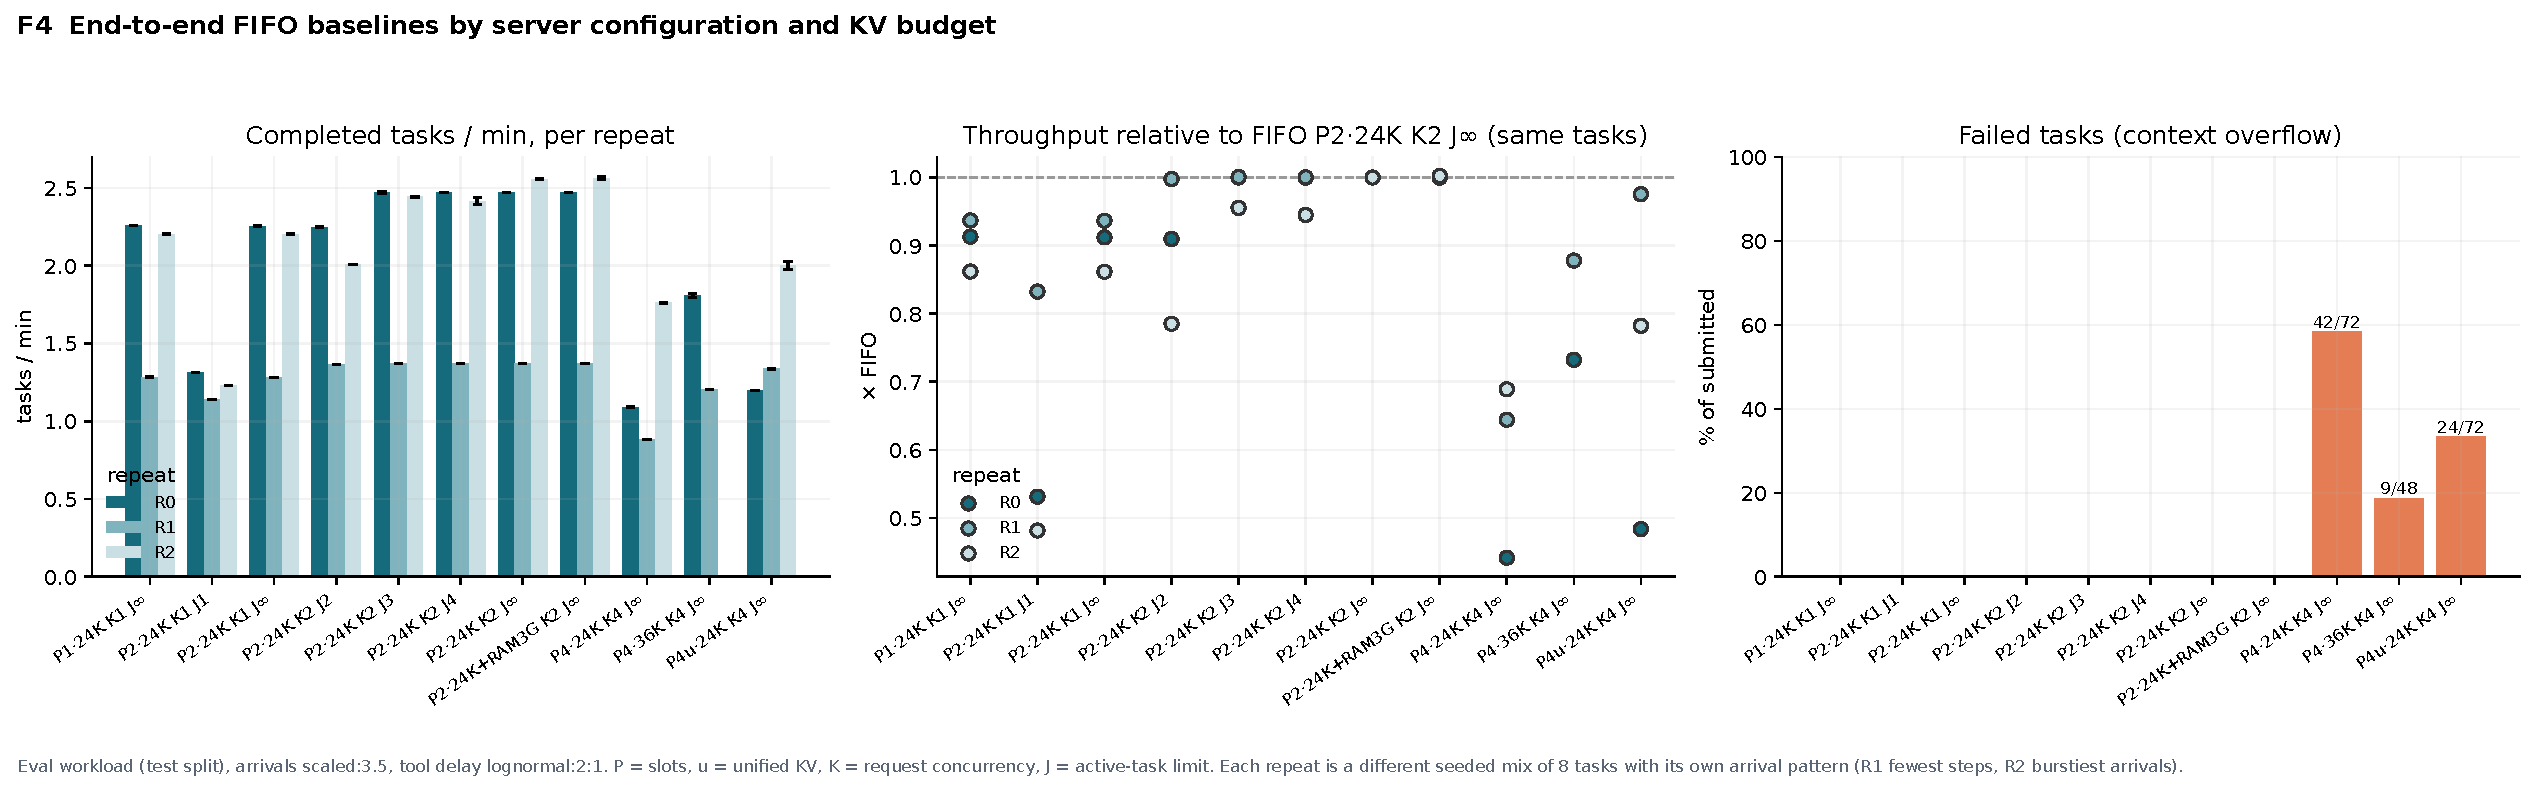
\includegraphics[width=\textwidth]{t4_f04_main.pdf}
\caption{Baselines on the M4 (top) and the T4 (bottom), per repeat, relative to FIFO on the same tasks.}
\end{figure}

\begin{figure}[h]
\centering
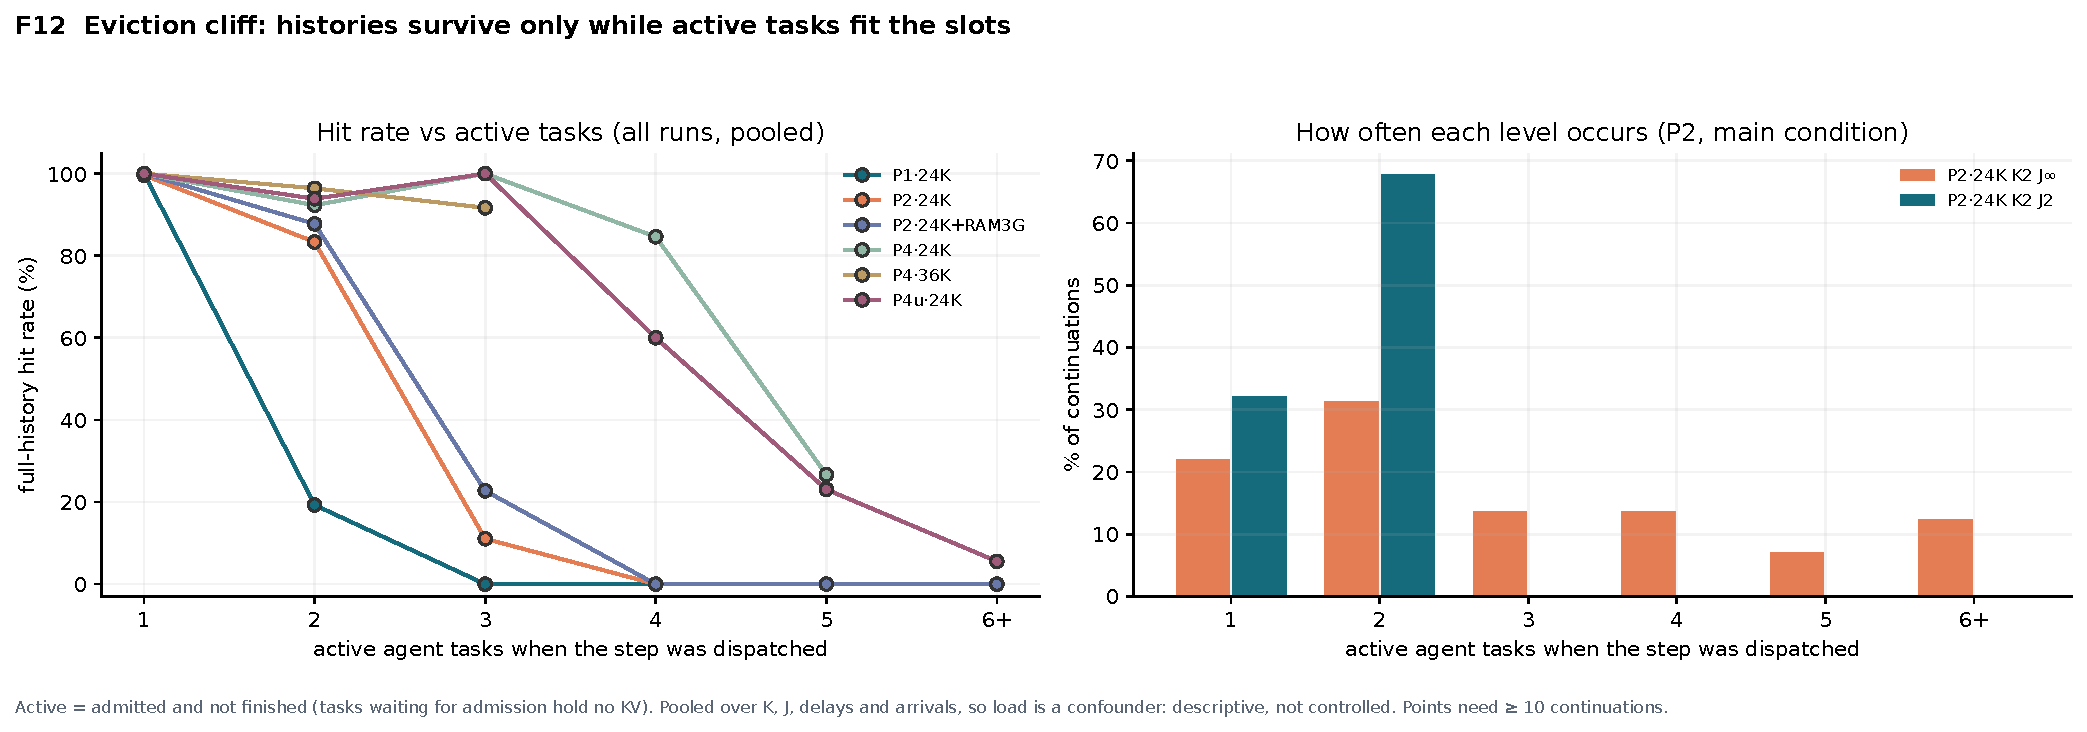
\includegraphics[width=\textwidth]{m4_f12_eviction.pdf}
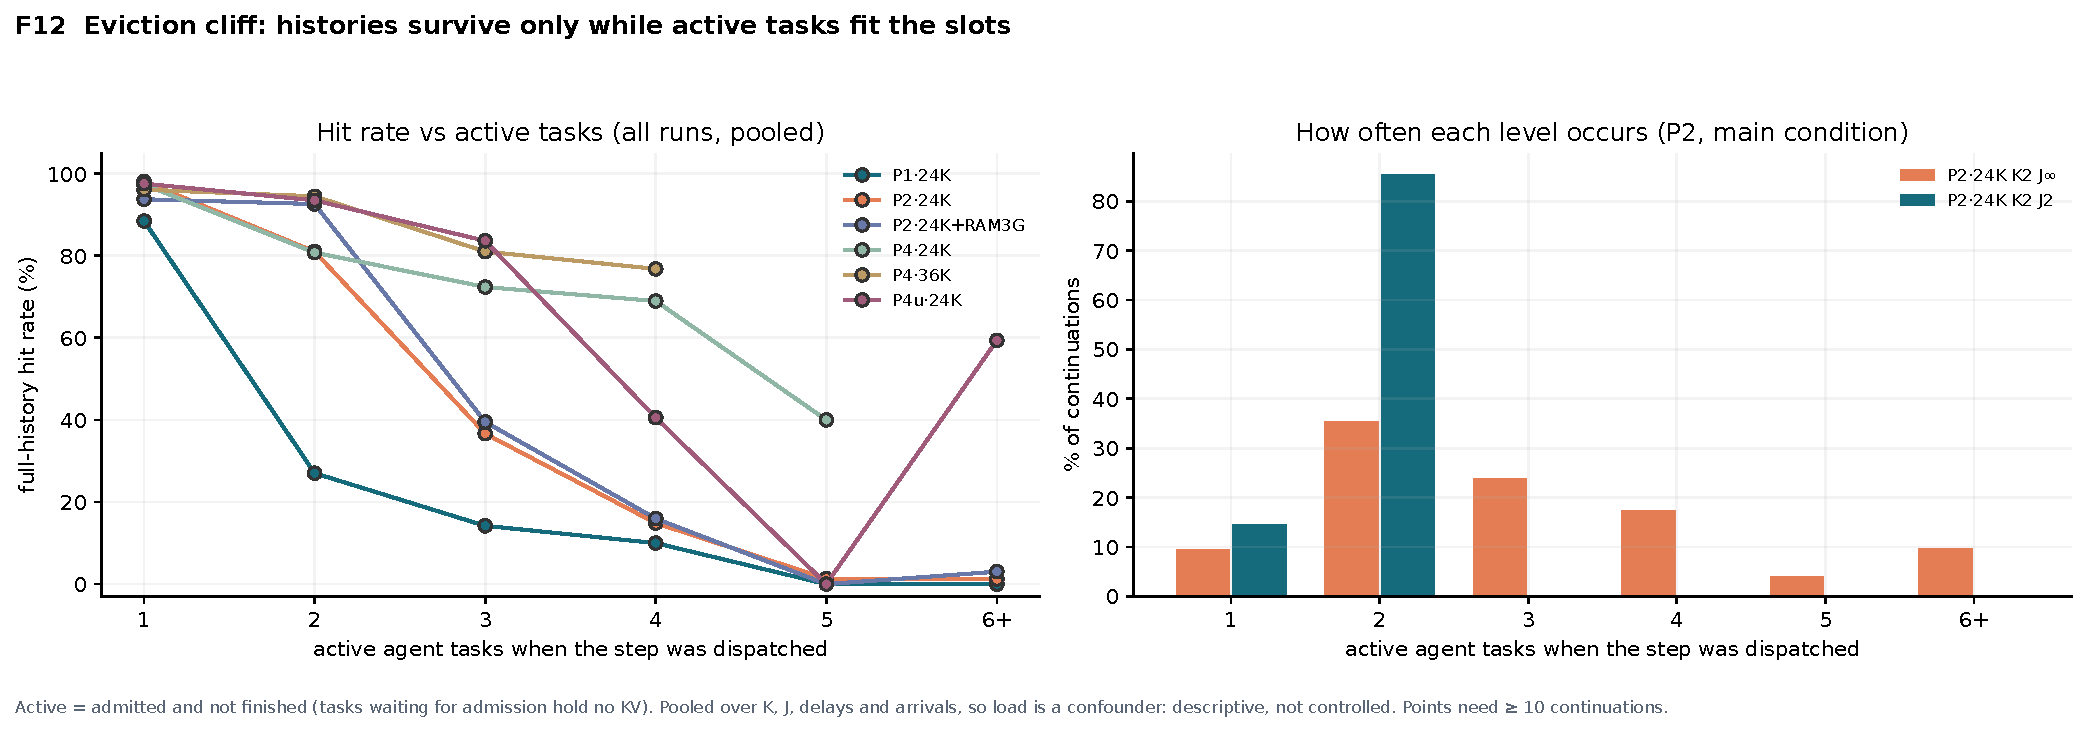
\includegraphics[width=\textwidth]{t4_f12_eviction.pdf}
\caption{Eviction cliff on the M4 (top) and the T4 (bottom): histories survive only while active tasks fit the slots.}
\end{figure}

\begin{figure}[h]
\centering
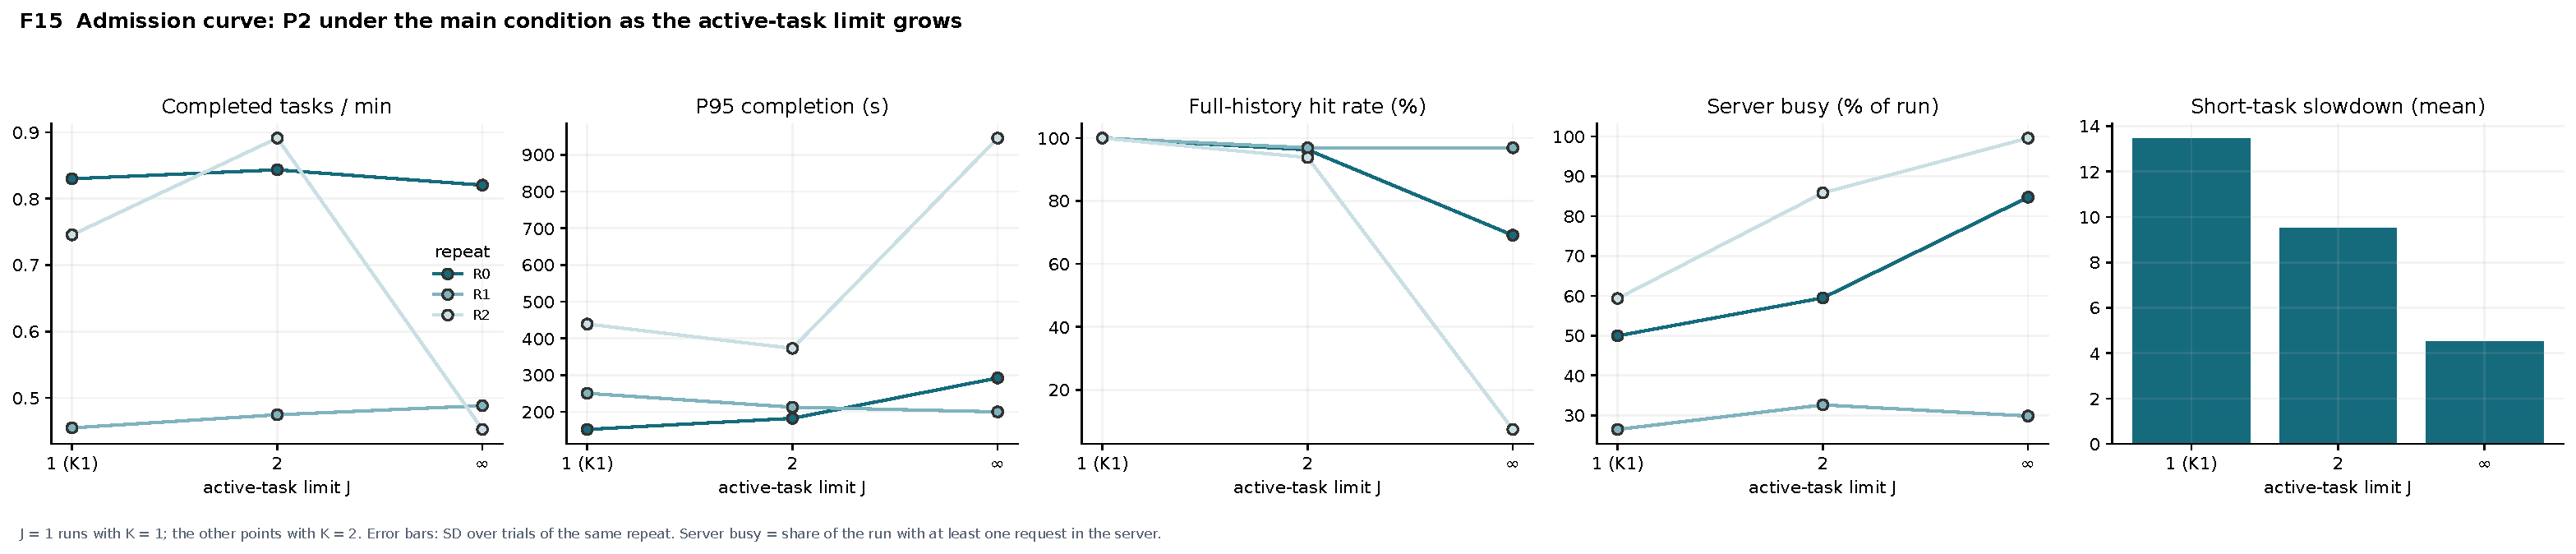
\includegraphics[width=\textwidth]{m4_f15_admission.pdf}
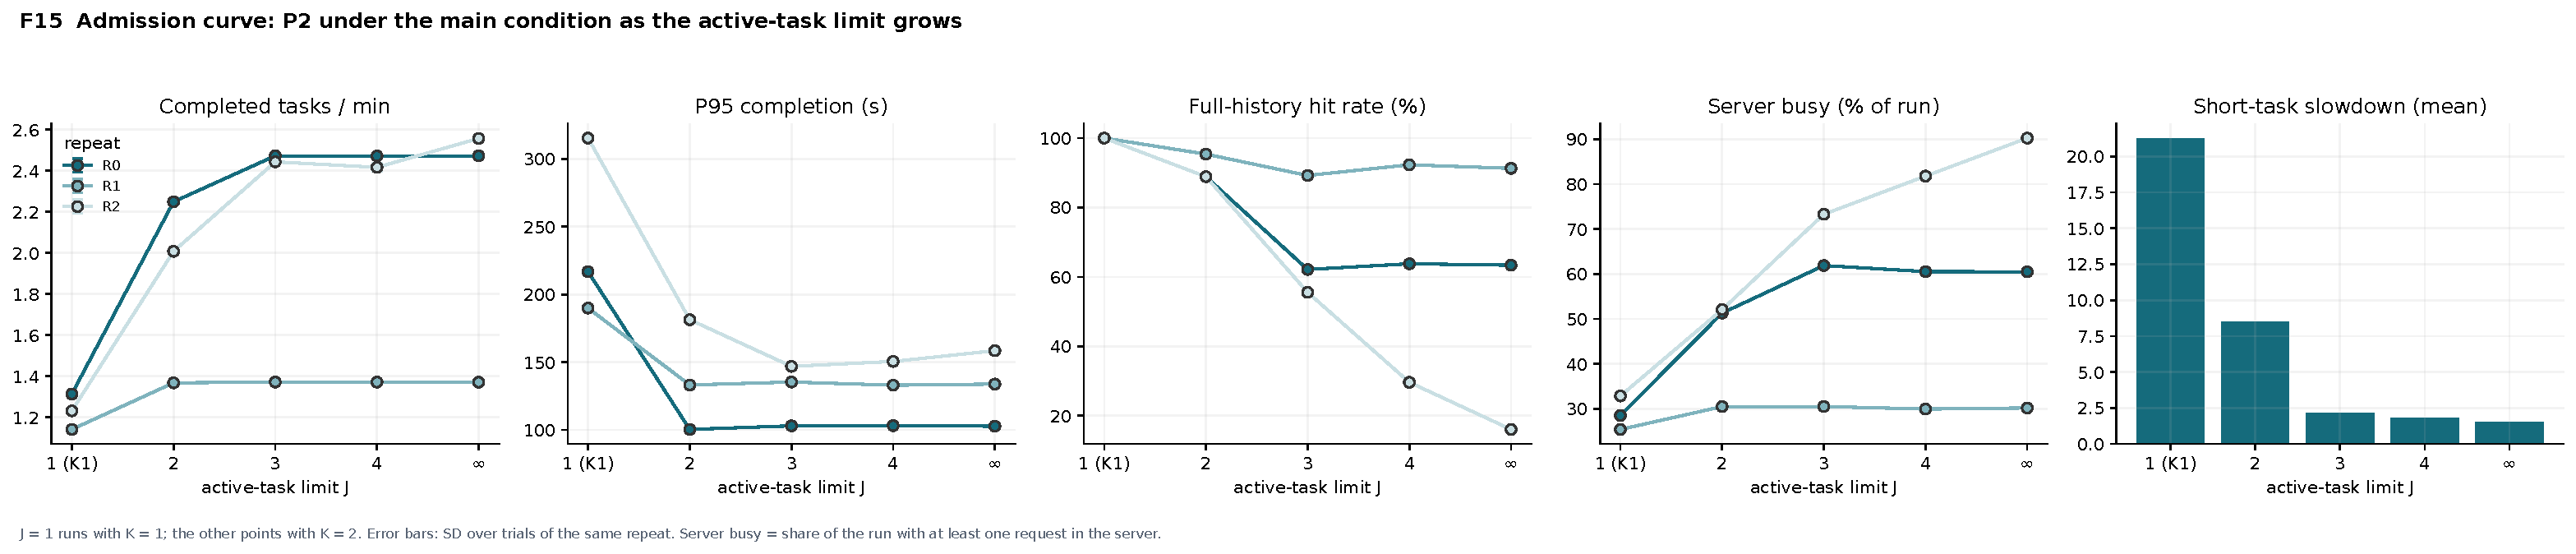
\includegraphics[width=\textwidth]{t4_f15_admission.pdf}
\caption{Admission curves on the M4 (top) and the T4 (bottom). On the M4 throughput peaks at $J=2$; on the T4 it keeps rising with $J$ as the server stays busier.}
\end{figure}

\begin{figure}[h]
\centering
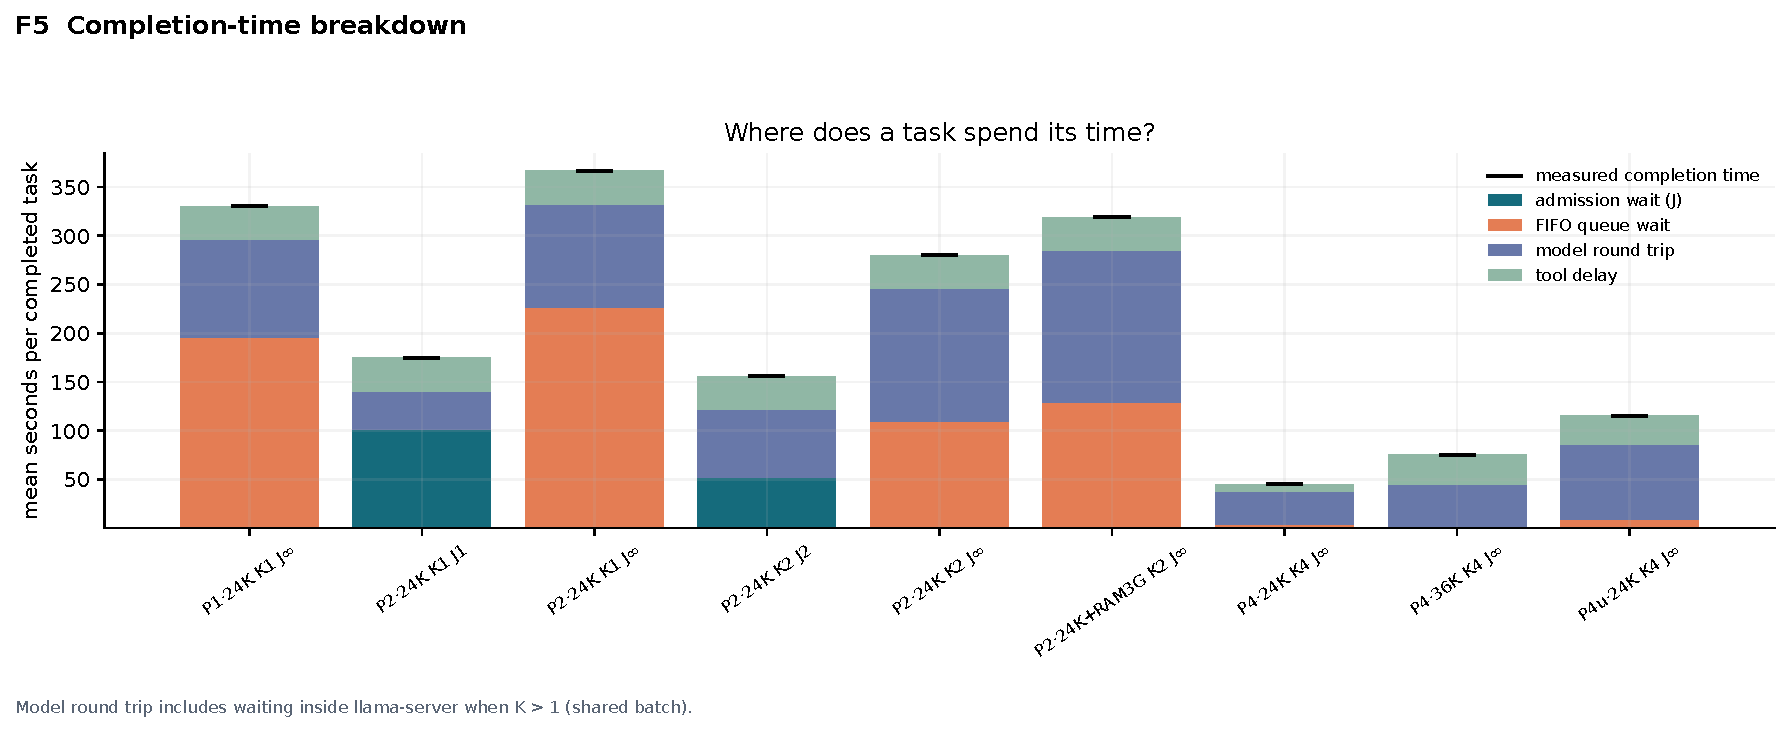
\includegraphics[width=\textwidth]{m4_f05_breakdown.pdf}
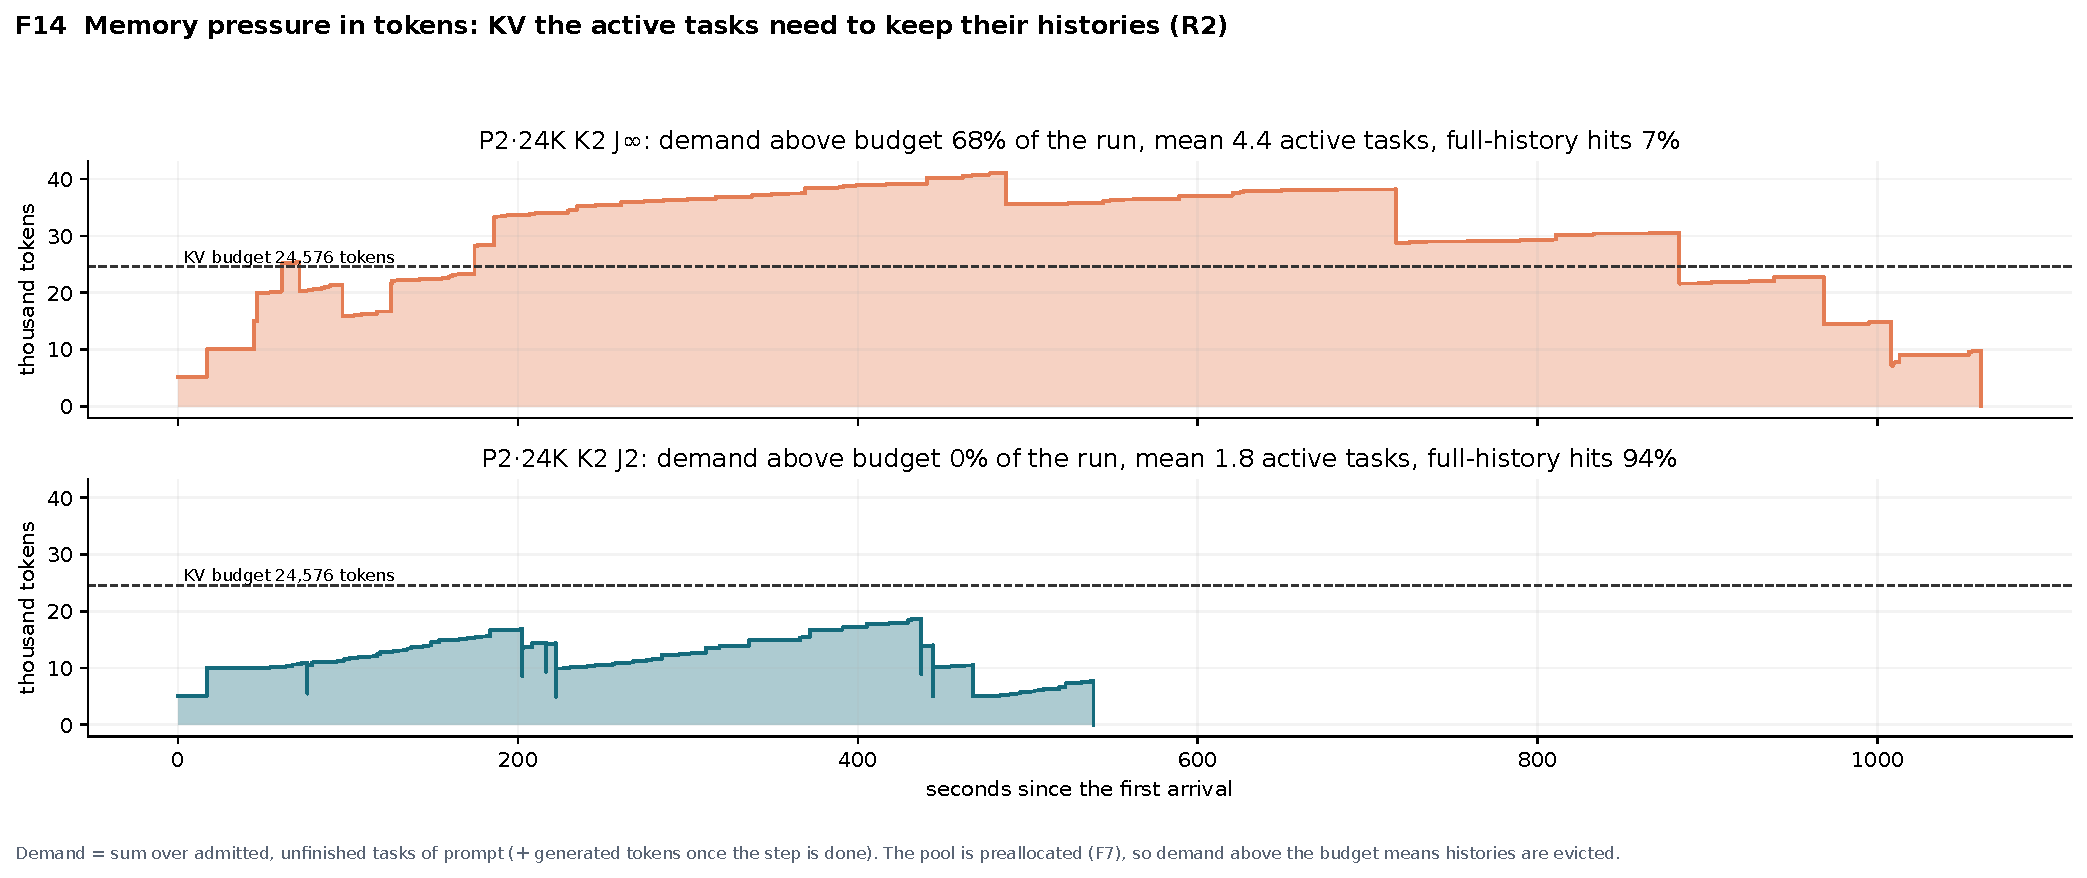
\includegraphics[width=\textwidth]{m4_f14_kv_demand.pdf}
\caption{M4 time per completed task, and KV demand of the admitted tasks against the 24K budget.}
\end{figure}

\begin{figure}[h]
\centering
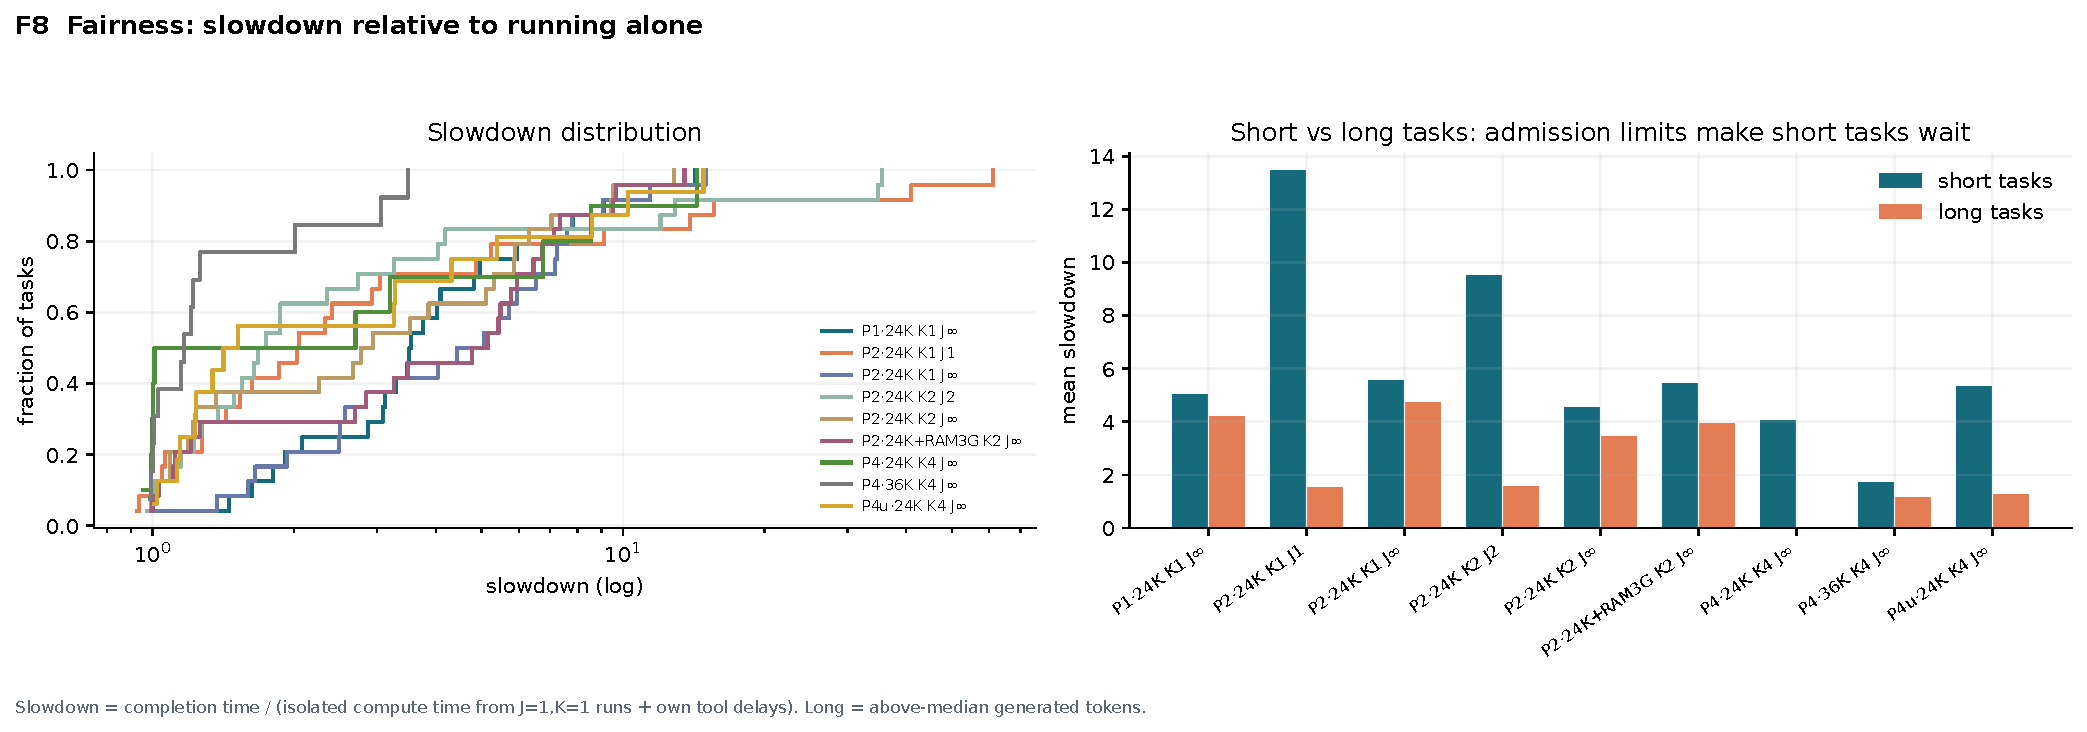
\includegraphics[width=\textwidth]{m4_f08_fairness.pdf}
\caption{M4 slowdown of short and long tasks.}
\end{figure}

\begin{figure}[h]
\centering
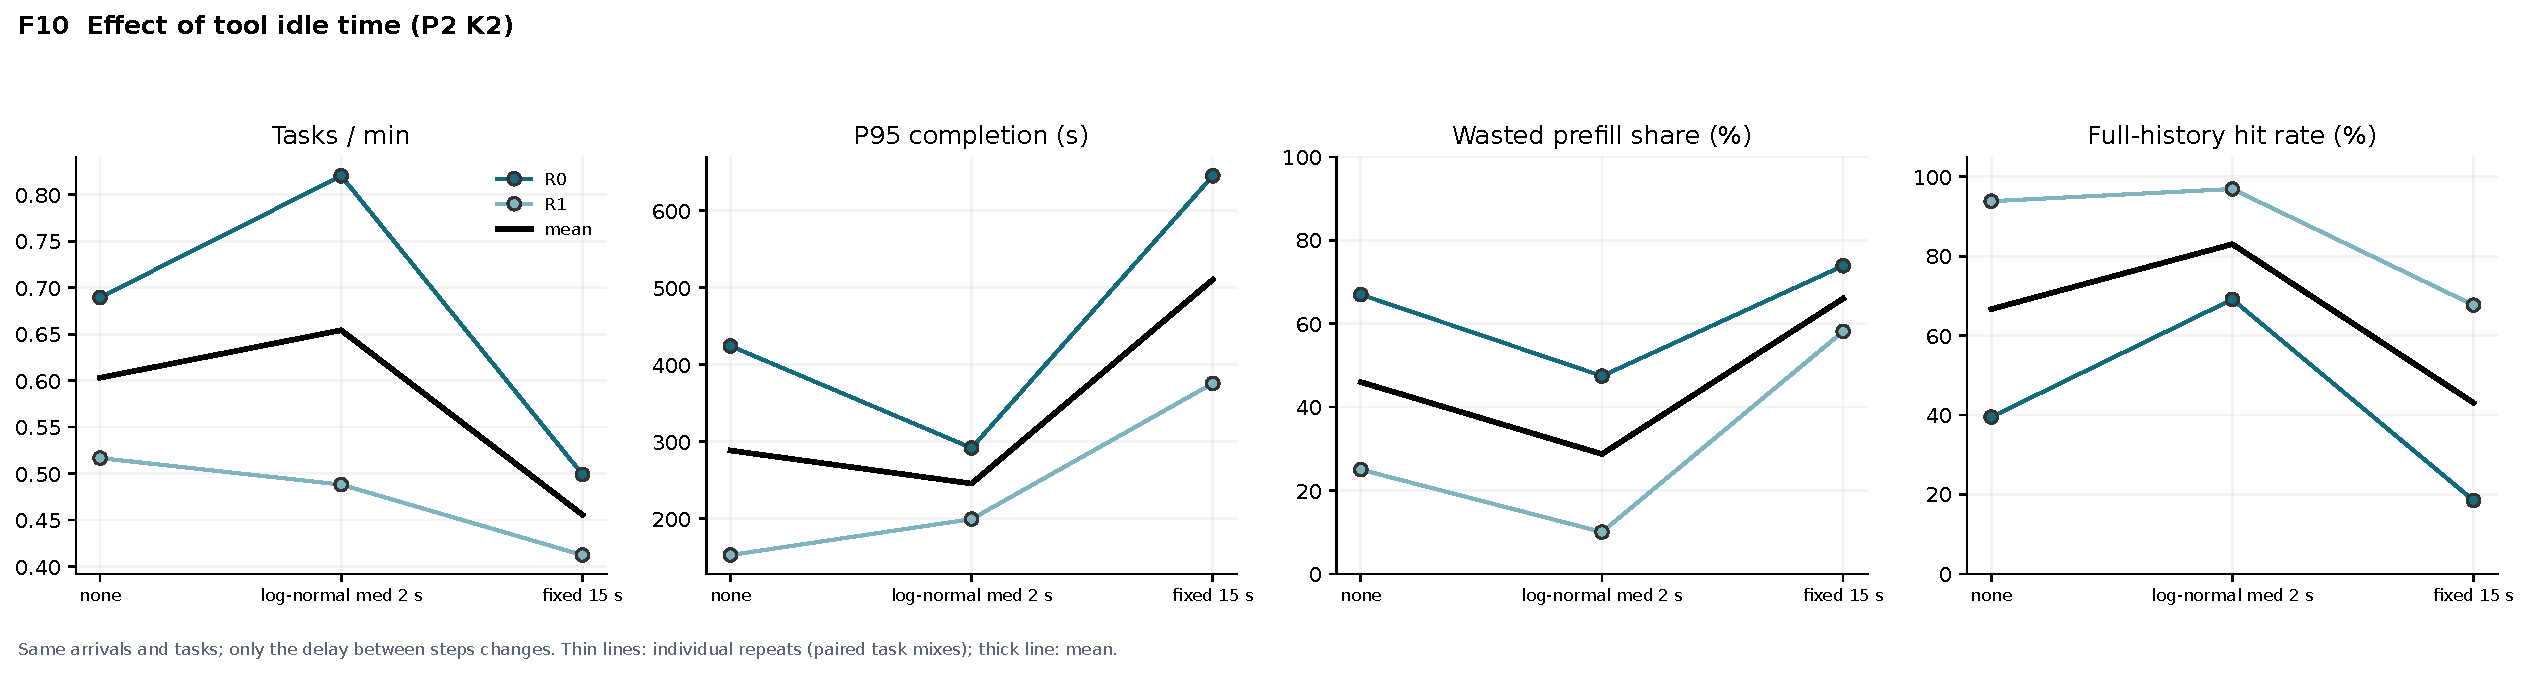
\includegraphics[width=\textwidth]{m4_f10_tool_delay.pdf}
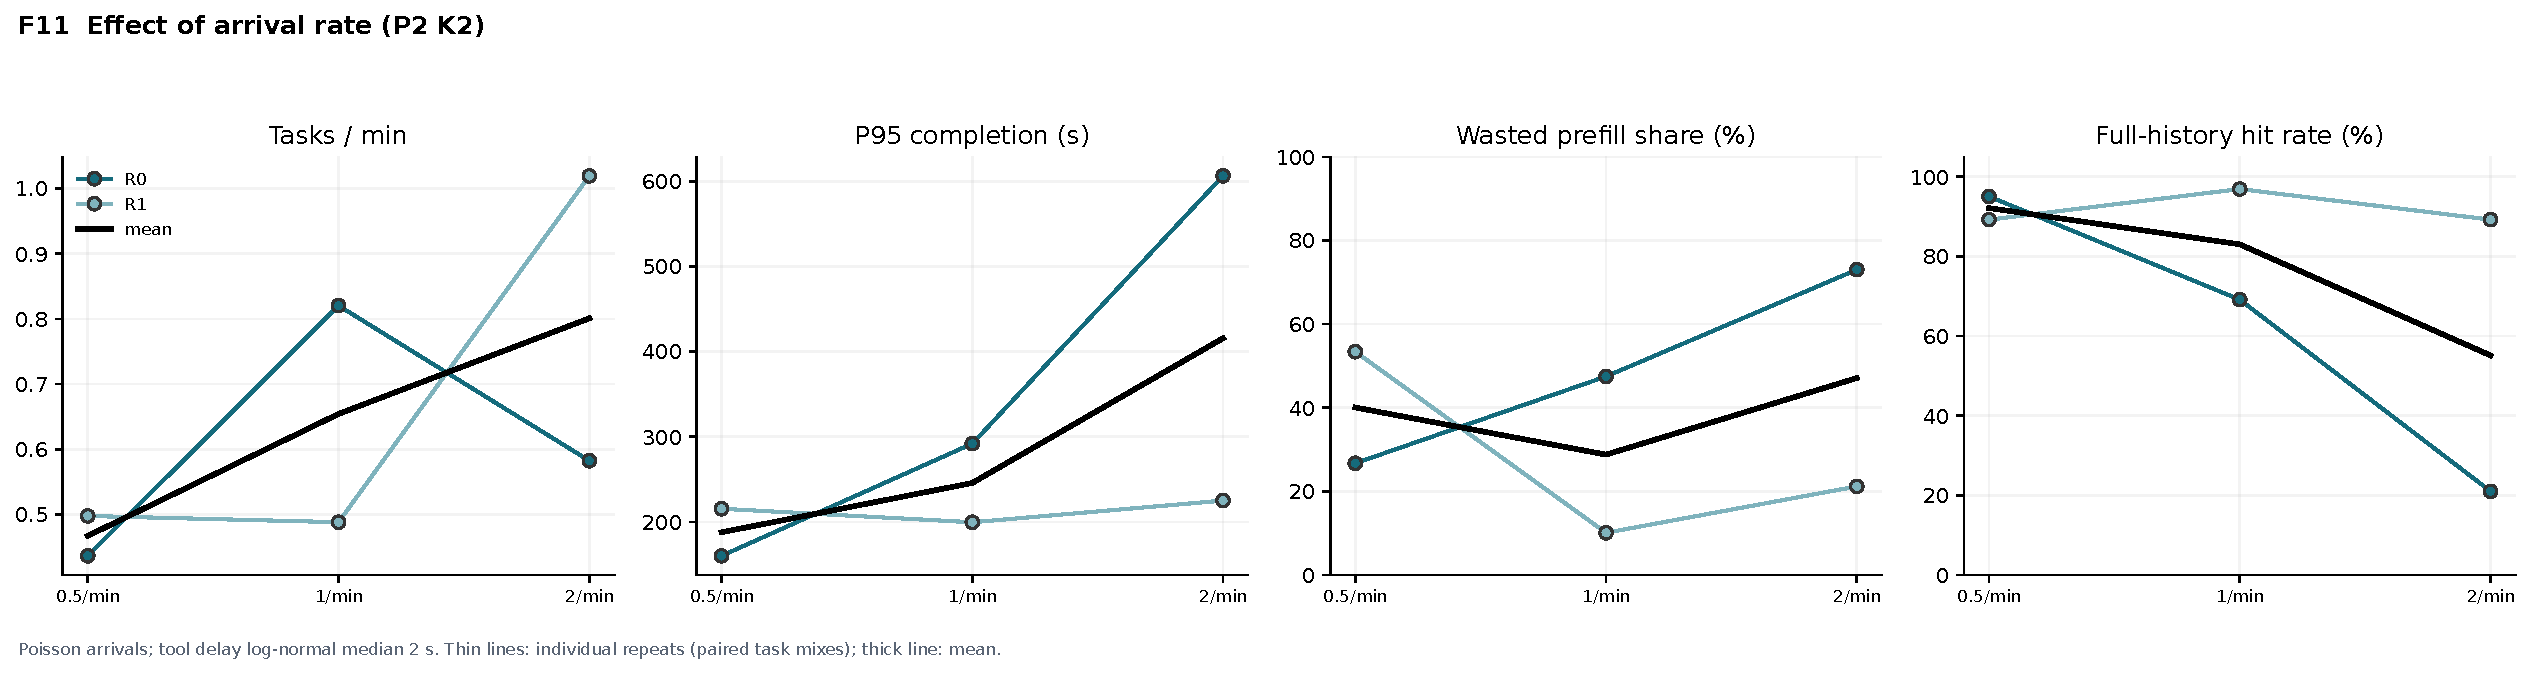
\includegraphics[width=\textwidth]{m4_f11_arrival.pdf}
\caption{M4 tool-delay and arrival-rate sweeps ($P=2$, $K=2$), compared on the repeats that every setting ran.}
\end{figure}

\begin{figure}[h]
\centering
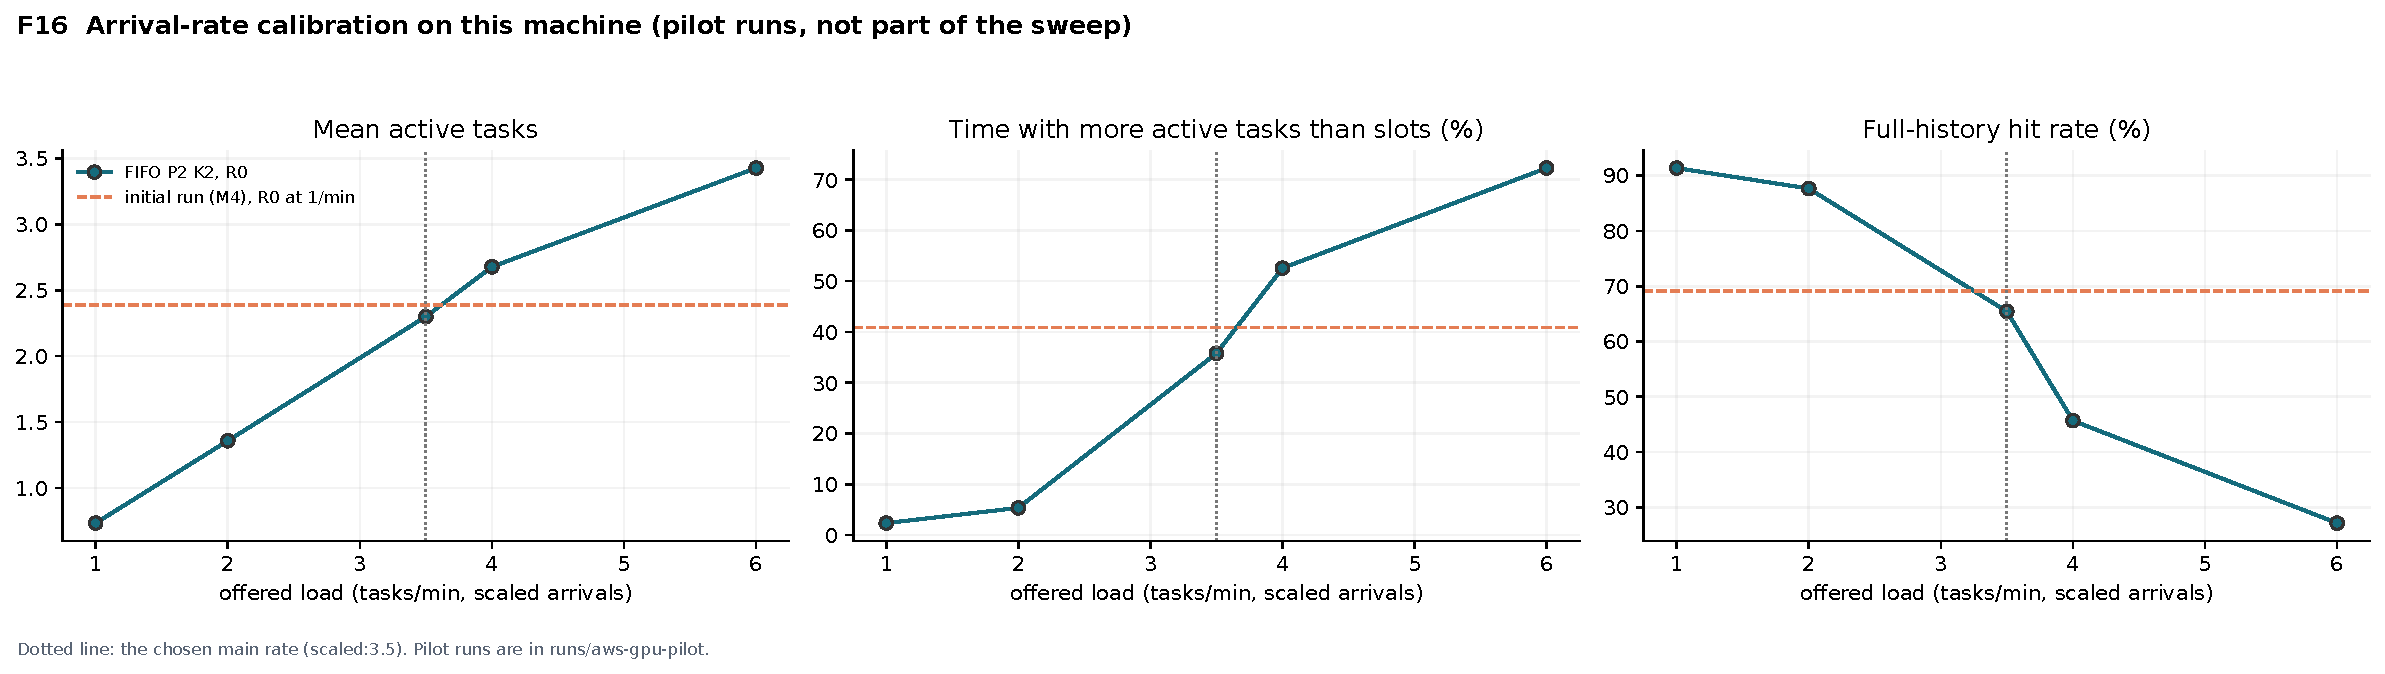
\includegraphics[width=\textwidth]{t4_f16_calibration.pdf}
\caption{T4 arrival-rate calibration: 3.5 tasks/min matches the M4's FIFO contention on R0.}
\end{figure}

\clearpage
\section{Timeline}

\textbf{Done}
\begin{itemize}
\item October 16. We wrote a design memo that treats queue priority and cache retention as one loop. The score and the retention formula in that memo were a plan, and they are not in the code.
\item October 16 to 26. We built the FIFO, captured the live Retail tasks, made the append-only replay, and ran the micro benchmark, the cache probe, the restore check, and the M4 eval and dev sweeps.
\item October 26. Figures and the generated numeric report.
\item October 28 to November 3. M5 noise trials, T4 arrival-rate calibration, and the T4 eval and dev sweeps with three trials of every run.
\item November 4. This writeup.
\end{itemize}

\textbf{Phase 2}
\begin{itemize}
\item November 11. Add slot pinning on the current runner, and on the dev split check that a second slot is actually used at $K = 1$.
\item November 18. Add a continuation-first queue with aging and cost-based admission for new tasks, and compare it on dev with the best fixed cap of each machine.
\item November 25. While a tool runs, choose pin, SSD save, or evict from the costs measured here, and log the decision time and the save time.
\item December 2. Run the eval comparison on the M4 and the T4: FIFO, the best fixed baseline, the host cache, queue only, cache only, and both. Include 0.5 arrivals per minute and zero tool delay, and report short-task and long-task slowdown.
\item December 8. Freeze the commit, rerun any number the report states, and draft the 4 to 6 page final report.
\item December 10. Submit the scheduler, the runner, the raw logs, the analysis scripts, and the final report.
\end{itemize}

\end{document}
